%&header
% !TeX root = 1_introduction

\input{build/subheader.tex}
\endofdump

\ifRootBuild\else
  \newglossaryentry{ASIC}{name={ASIC},
                  description={Application Specific Integrated Circuit} } 
                  
\newglossaryentry{ATR}{name={ATR},
                  description={Automatic Target Recognition} } 

\newglossaryentry{CPU}{name={CPU},
						description={Central Processing Unit} } 

\newglossaryentry{GPGPU}{name={GPGPU},
						description={General Purpose Graphics Processing Unit} } 

\newglossaryentry{GPU}{name={GPU},
						description={Graphics Processing Unit} } 
					
\newglossaryentry{MVDR}{name={MVDR},
						description={Minimum Variance Distortionless Response} } 
  \makeglossaries
\fi

%\beforeepigraphskip

\begin{document}


\newcommand\chapref[2]{\hyperref[#1]{#2.\ref{#1}}}

\chapter{Background}

{

% \newcommand\mat[1]{\boldsymbol{#1}}
\newcommand\bmat[1]{\begin{bmatrix}#1\end{bmatrix}}
\renewcommand*\eR{\mat{\hat R}}
\renewcommand\1{\vec 1}

\section{Introduction}

% Graphics Processing Units (GPUs) is a technology tailored to perform image processing as fast as possible. They are available off-the-shelf at reasonable prices, are very power efficient, and can be programmed to carry out a wide range of computational tasks, often displaying speed increases of an order of magnitude compared to similar CPU designs. Initially, GPUs may seem perfectly suited for image reconstruction algorithms, because usually each pixel can be computed independently and concurrently of one another. While this is true for simple techniques such as conventional beamformers, the more complex per-pixel computations present in adaptive techniques are harder for the GPU to handle.
% 
% Through a case study of on such technique, the Minimum Variance Distortionless Response (MVDR) beamformer, we identify these challenges and explain how they were overcome. The MVDR technique is known for its notable potential for improving image quality over simple conventional methods, but it is also far more computationally complex. This is because a spatial covariance matrix must be estimated and inverted for each image pixel, the former dominating for systems with less than 20-30 channels, and the latter otherwise. 
% 
% We propose three different solutions to the complexity issue depending on system size. For smaller systems we use the standard time-domain MVDR method, arithmetically optimize the estimation step, and show that image creation rates of more than 1\,Mpx/s can be achieved when this algorithm is run on a GPU. For medium sized systems we suggest applying the MVDR in the beamspace (frequency domain) instead, which allows for comparable processing rates at a negligible reduction in image quality. Finally, for large systems the estimation and inversion step can be avoided completely by utilising the Low Complexity Adaptive (LCA) beamformer.\todo{disse tre første avsnittene burde sikkert vært kortet ned mye men...}
% 
% 
% The end design is more than 2 orders of magnitude faster than a C implementation we started off with, it took considerable effort to get there.
% \\
% << MOTIVATION >>
% \\

% Related work can be found e.g. in ultrasound imaging, where Chen et. al have investigated porting a time domain MVDR method to a GPU \cite{Chen2009,Chen2011,Chen2011a}. Unlike their work, however, we do not impose the restriction of the input data to be real, nor do we approach larger systems by enforcing Toeplitz structure of the covariance matrix. 
% \\

Any wave, regardless of its nature, is governed by a partial differential equation known as the \emph{wave equation}:
%
\begin{align}
\nabla^2 f 
 = \frac{1}{c}\frac{\delta^2 f}{\delta t^2},
\end{align}
%\frac{\delta^2 f}{\delta x^2} + \frac{\delta^2 f}{\delta y^2} + \frac{\delta^2 f}{\delta z^2}
%
where $\nabla^2$ is the Laplace operator, $f$ is field strength and $c$ is wave propagation speed. If $f$ represents the displacement of a vibrating string, the equation states that the force pulling the string towards equilibrium (right side) is proportional to the string's curvature (left side). In acoustics $f$ represents sound pressure, but since the mathematics are independent of the physics involved we will simply think of $f$ as a signal: a unit-less scalar function with wave characteristics.

The wave equation has a few solutions of interest, in particular that of a plane and spherical wave:
%
\begin{align}
f_\textrm{plane}(\vec{p},t)  &= A e^{j(\omega t - \vec{k} \cdot \vec{p})} \\
f_\textrm{spheric}(\vec{p},t) &= \frac{A}{\lVert \vec{p} \rVert} e^{j(\omega t - \lVert\vec{k}\rVert \lVert \vec{p} \rVert)},
\end{align}
% 
Here $A$ is amplitude, $\omega$ is temporal wave frequency, $t$ is time, $\lVert\vec{k}\rVert=\frac{\omega}{c}=\frac{2\pi}{\lambda}$ is spatial wave frequency (wavenumber) and $\vec{p}$ is position of the source relative to the observer. 

% One is that of plane wave and the other a  A signal source with the position $\udot{S}$ . We can represent the field observed at $\udot{A}$ as $f(\dvec{p}^A,t)$, where position is represented by $\dvec{p}^A=[x_A,y_A,z_A]^T\in\mathbb{R}^3$ and time by $t\in\mathbb{R}$,
% 
% An introduction to such notation can be found in \chapref{IV_methods}{IV}.
% 
% 
% reference frame $\ubar{A} \triangleq (\udot{A},\uvec{A})$ to it, where $\udot{A}\in\mathbb{A}$ is its absolute position and $\uvec{A}\triangleq\big(\hat{x}_{A},\hat{y}_{A},\hat{z}_{A}\big)\in\mathbb{V}^3$ its absolute orientation (where $\hat{\cdot}$ denotes unit length)


%

%
% \hyperref[IV_methods]{\chapterref{IV_methods}.\sectionref{IV_methods}}
% \renewcommand{\thesection}{\thechapter.\arabic{section}}

% Suppose an array of sensors has a reference frame $\ubar{A} \triangleq (\udot{A},\uvec{A})$ attached to it, where $\udot{A}\in\mathbb{A}$ is its absolute position and $\uvec{A}\triangleq\big(\hat{x}_{A},\hat{y}_{A},\hat{z}_{A}\big)\in\mathbb{V}^3$ its absolute orientation (where $\hat{\cdot}$ denotes unit length). 


% This article is outlined as follows: First we will present the mathematical formulation and evaluate complexity aspects of the MVDR method operated in time or frequency domain, and on the LCA beamformer. Then we mention some of our experiences with implementing the MVDR on a GPU, before concluding with some results and final thoughts.


\section{Image reconstruction}\label{methods}

Consider an acoustic signal transmitted to highlight a surface of interest. Assume the backscattered wavefield is properly sampled using a uniform linear array (ULA) of receivers. After stripping the carrier frequency by heterodyning and the signal signature by matched filtering (Fig. \ref{I_beamforming}), an image is formed by coherently combining the receiver outputs to focus at one angle (or point) at a time. The principle of adjusting the array's focus in range and direction is commonly referred to as beamforming, and involves assigning suitable delays and weights to the array's channels.

\begin{figure}[tp]\label{II_fig_article_relation}
\makebox[\linewidth][c]{%
\graphicsAI[drawing,width=1.3\linewidth]{gfx/article_relation.svg}}
\caption{Method relations. This thesis explores three beamformers reconstructing images from acoustic echoes: time-domain MVDR (reference), frequency-domain MVDR (close approximation) and time-domain LCA (educated trial-and-error). Background on synthesis of image templates from the reconstructed images will be presented in article IV. }
\end{figure}

\subsection{Beamforming}
% \ifPhdDoc
% \begin{figure}[htbp]\centering
% \includegraphics[width=\linewidth]{gfx/buske1\figPostfix.eps}
% \else
% \ifPeerReview
% \begin{figure}[htbp]\centering
% \includegraphics[width=0.8\linewidth]{gfx/buske1\figPostfix.eps}
% \else
% \begin{figure}[!t]\centering
% \includegraphics[width=\linewidth]{gfx/beamforming.eps}
% \fi\fi%
% \caption{Beamforming principle. Signal signature is first removed by matched filtering. Then, before summation, a suitable set of delays $\Delta$ and weights $w$ are applied to focus on a pixel of interest at angle and range ($\theta,n$).}\label{I_beamforming}
% \end{figure}

Imagine an array with $M$ sensors with a reference frame $\ubar{A} \triangleq (\udot{A},\uvec{A})$ attached to it, where $\udot{A}\in\mathbb{A}$ is its absolute position and $\uvec{A}\triangleq\big(\hat{x}_{A},\hat{y}_{A},\hat{z}_{A}\big)\in\mathbb{V}^3$ its absolute orientation (where $\hat{\cdot}$ denotes unit length). Assume that the array channels are digitally delayed to focus at a pixel with azimuth angle $\theta$ and range sample $n$, such that the delayed data from the $m$th channel can be expressed as $x_m[\theta,n-\Delta_m]\in\mathbb{C}$. By making the dependence on $\theta$ implicit and assuming the data to be pre-delayed to the pixel of interest, we can simplify the notation to $x_m[\theta,n-\Delta_m] = x_m[n]$. 

The beamformer output $z[n]\in\mathbb{C}$ is by definition the weighted sum of all the delayed data samples:
%
\begin{align}
z[n] = \dvec{w}^H[n]\dvec{x}[n] = \bmat{w_0[n]\\w_1[n]\\\vdots\\w_{M-1}[n]}^H \bmat{x_0[n]\\x_1[n]\\\vdots\\x_{M-1}[n]} \in\mathbb{C},\label{2_eq_z}
\end{align}
%
where $w_m\in\mathbb{C}$ is the weight factor assigned to channel $m$. With static weights this is referred to as the conventional delay-and-sum (DAS) beamformer. A variety of weighting functions exist for trading lateral resolution for improved noise suppression (contrast), but a compromise between the two is unavoidable~\cite{Harris1978}. A class of adaptive beamformers target this limitation by adapting the weights to the impinging wavefield. One such technique is the minimum variace distortionless response (MVDR) method.



% Accelerated adaptivity is key: it enables rapid dynamic responses to mission events. }


\subsection{Time-domain MVDR}

\begin{figure}[t]\centering%
\graphicsAI[drawing,width=1\linewidth]{gfx/implementation.svg}%
\caption{MVDR beamforming. For one of the total number of pixels in range and azimuth, $N_y$ and $N_x$,\newline
1. an $L\times{}L$ sample covariance matrix $\eR$ is computed, \newline
2. the term $\eR^{-1}\1$ is found using a linear equation solver,\newline
3. and the beamformer output is computed from $z$ from (\ref{finalZ}), where $\w$ is found by substituting $\eR^{-1}\1$ into (\ref{2_eq_weights}). }\label{mvdr_beamforming}
\end{figure}
%
The basic idea behind MVDR is to compute the set of weights that minimizes noise and interference accumulated by the array, while ensuring unit gain for signals coming from the pixel of interest. With pre-delayed data this can be formulated as follows:
%
\begin{gather}
\argmin{\dvec{w}}\ E\Big\{\big|\dvec{w}^H[n]\dvec{x}[n]\big|^2\Big\} \qquad\text{subject to}\qquad \dvec{w}^H[n]\dvec{1} = 1. \label{2_eq_mvdr_def}
% \vec w[n] = \frac{\Ri[n]\1}{\1^T\Ri[n]\1},\label{2_eq_weights}
\end{gather}
%
This optimization problem has the solution:
%
\begin{gather}
\vec w[n] = \frac{\Ri[n]\dvec{1}}{\dvec{1}^T\Ri[n]\dvec{1}},\label{2_eq_weights}
\end{gather}
%
where $\dvec1$ is a row vector of ones representing broadside steering and $\R=E\{\x[n]\x^H[n]\}$ is the spatial covariance matrix for the full array. We estimate $\R$ by computing a sample covariance matrix $\eR$. A good estimate requires some degree of \emph{spatial averaging} to avoid signal cancellation, \emph{temporal averaging} to maintain true speckle statistics, and \emph{diagonal loading} to improve robustness to parameter errors ~\cite{Synnevag2009a}. Combined, these techniques will also ensure a numerically well conditioned $\eR$. 

To arrive at a formulation of how $\eR$ can be estimated, we first split the array into subarrays of length $L$ that overlap on all but one sensor. If we let $x_l[n]$ represent the datavector from subarray $l$,
%
\begin{gather}
\dvec{x}_l[n] = \bmat{x_l[n] & x_{l+1}[n] & \dots & x_{l+L-1}[n]}^T.
\end{gather}
%
then the sample covariance matrix formed with temporal and spatial averaging, $\eR$, is given as:
%
\begin{gather}
\eR[n] =  \frac{1}{N_K N_L} \sumb{l=0}{N_L-1}\sumb{n'=n-K}{n+K} \x_l[n]\x_l^H[n] \in\mathbb{C}^{L,L},\label{2_eq_spatialR}
\end{gather}
%
where $N_K = 2K+1$ is the number of temporal samples to perform averaging over, and $N_L = M-L+1$ is the number of subarrays. In the actual design a fraction of the total power of $\eR[n]$ is finally added to its diagonal~\cite{Synnevag2007}, but this step will be ignored here due to its negligible contribution to runtime.

To summarize as in Figure \ref{mvdr_beamforming}: For every pixel in the image we estimate $\eR$ (\ref{2_eq_spatialR}), solve the linear equation $\eRi\1$ (\ref{2_eq_weights}), the finally substitute some to get the beamformer output (\ref{2_eq_mvdr_def}-\ref{2_eq_weights}).



\subsection{Frequency-domain MVDR}

Above 32 channels the inversion step becomes a greater computational bottleneck than covariance estimatation. We mitigate this by applying space reduction in the spatial frequency-domain, or beamspace. If the data is narrow band, narrow beam, or both, the backscatter energy resides primarily in the center frequencies. The zero-frequency correspond to broadside, higher frequencies to larger opening angles. Since the combined transmit and receive response is highly directive, it is sufficient to process only three or five center angles and ignore the rest~\cite{Nilsen2009a,VanTrees2002}. The method is called beamspace MVDR.

Beamspace MVDR formulation closely resembles that of time domain MVDR, the main difference being an initial need to Fourier transform the data:
%
\begin{gather}
\x_{\text{BS},l}[n] = \mat{B}\x_l[n], \qquad \mat{B}\in \mathbb{C}^{N_b,L}, \qquad \text{where} \qquad [\mat{B}]_{p,q} = \frac{1}{\sqrt{L}} e^{-j2\pi\,p\,q/L}.\label{2_eq_beamspace}
\end{gather}
%
Here $\mat{B}$ refers to the Butler matrix, $l$ is subarray index, and $N_b$ is number of beams that should be computed. Note has once $\x_{\text{BS},l}[n]$ is computed, $\eR_\text{BS}$ can be found as in (\ref{2_eq_spatialR}), $\w_\text{BS}$ as in (\ref{2_eq_weights}), and $z$ as in (\ref{z}).

Reducing the covariance size from $L$ to $N_b$ also reduce the estimation step to O($N_K N_L N_b^2$), and the inversion step to O($N_b^3$). The downside is the additional computations required by the frequency transform, which must be weighted up against the gain of reducing $N_b$.



\subsection{LCA beamformer}

The Low Complexity Adaptive (LCA) beamformer offers a different approach to the optimization problem in (\ref{2_eq_mvdr_def}). Instead of calculating weights like MVDR in (\ref{2_eq_weights}), it iterates through a set of precomputed weights and applies the one that best fulfils the optimization criterion. If $\w_p$ denotes the $p$'th out of $P$ weight sets, then LCA can be formulated as~\cite{Synnevag2008}:
%
\begin{gather}
\argmin{p}\ E\Big\{\big|\w_p^H\x[n]\big|^2\Big\} \qquad\text{subject to}\qquad \w_p^H\1 = 1. \label{2_eq_lca_def}
\end{gather}
%
Note the similarity between (\ref{2_eq_mvdr_def}) and (\ref{2_eq_lca_def}). Both LCA and MVDR rely on the same optimization criterion, but whereas MVDR searches a continuous solution space for the optimal weights, LCA only have $P$ solutions to select from.



% \subsection{Image quality}


% These challenges are very closely linked. The Quadro 6000 architecture is of compute capability 2.0, which means there are 48\,kB of shared memory (L1 cache) and 128\,kB of registers per SM~\cite{Nvidia2012}. This memory is shared by all active threads on that SM, a number that should be no less than 768~\cite{Nvidia2012a}. This will expose a sufficient level of data parallelism to ensure that memory latency is completely hidden (Little's law). By dividing the shared memory evenly on all 768 threads we find that each thread should store no more than 8 single precision complex numbers in shared memory\todo{introduce memory structure -shared for data shared between threads}, and 24 stored in registers. This should make it apparent why computing a single pixel per thread is a bad idea, and why we need to keep each thread as light on memory consumption as possible.

% Most of the challenges we faced when porting the MVDR to a GPU are caused by a single troublesome fact: GPU prefers threads that computationally intensive but very light on memory consumption. 



% The solution is make sure that each thread primarily access the shared memory (L1 cache) and registers. Unfortunately, these are scarce resources and 

% \begin{figure}[!t]\centering\label{2_fig_holmengraa}%
% \graphicsAI[drawing,width=\linewidth]{gfx/plot_holmengraa_L16_Navg1.pdf}%
% \caption{The 68$\times$9\,m oil tanker Holmengraa lying at a depth of 77\,m. The MVDR images were processed with L=16, K=3, and 1\% diagonal loading. For beamspace MVDR we set $N_b=L/2$. LCA was set up with a window database consisting of 5 Kaiser windows with the window-parameter set in the range $\beta\in[0,10]$, and then each of these were steed in 5 distinct directions leaving a total of 25 windows for the LCA to select from..}
% \end{figure}
% 
% \begin{figure}[!h]\centering%
% \graphicsAI[drawing,width=.8\linewidth]{gfx/benchmark1_tagged.pdf}%
% \caption{Benchmarks for the our time-domain and frequency-domain MVDR method running on a GPU. The grey line marks the realtime requirement for the HUGIN AUV to perform full-coverage sectorscan images with a ping rate of 3 pings/s.}\label{2_fig_benchmark}
% \end{figure}
% 
% \section{Comparison}
% 
% Figure \ref{2_fig_holmengraa} contrasts image quality of the mentioned beamformers. The experimental data comes from a HISAS1030 interferometric synthetic aperture sonar (SAS) attached to a HUGIN autonomous underwater vehicle (AUV), both developed by Kongsberg Maritime, Norway. HISAS1030 is a fully digital phased array with 32 hydrophones, 100\,kHz center frequency, 30\,kHz bandwidth, 1.2\,m length, 23$^\circ$ half-power beamwidth (HPBW) and 3-4\,cm theoretical resolution both cross- and along-track. 
% 
% To display the imaging capabilities of the mentioned beamformers, we have processed experimental datasets from the 32 element Kongsberg Maritime HISAS1030 sonar mounted on the HUGIN AUV~\cite{Hansen2009}. HISAS1030 is a high resolution synthetic aperture sonar with an array length of 1.2\,m and operating frequency of 100\,kHz, and it was operated in sidescan mode here. The studied object is the 1500 dwt oil tanker wreck Holmengraa. It is 68\,m long and 9\,m wide, and lies at a slanted seabed at 77\,m depth outside of Horten, Norway. The results are shown in Figure \ref{2_fig_holmengraa}. The MVDR images were processed with parameters $L$=16, $K$=3, and 1\% diagonal loading. For beamspace MVDR we set $N_b=L/2$. LCA was designed with a window database consisting of 5 Kaiser windows, each with different window-parameters from the range $\beta\in[0,10]$, and each steered in 5 distinct directions leaving a total of 25 windows for the LCA to select from.
% 
% A few benchmarks of these methods are presented in Figure \ref{2_fig_benchmark}. On our test system with a quad-core Intel Xeon E5620, 64Gb of RAM and an nVidia Quadro 6000 card, the MVDR methods managed to create images at rates just over 1\,Mpx/s. A single-thread C implementation that was added as reference was outperformed by around 2 orders of magnitude. However, do not consider this comparison fair because while the GPU design is make efficient use of the L1 cache, similar optimisation work was not carried out on the CPU design.






% \begin{table}[h]\centering%\normalsize
% \begin{tabular}[c]{l r r r@{:}  l}\hline
% \rowcolor{tabBlue} & \multicolumn{1}{>{\columncolor{tabBlue}}c}{\bf BW$_\text{arithmetic}$} & \multicolumn{1}{>{\columncolor{tabBlue}}c}{\bf BW$_\text{memory}$} & \multicolumn{2}{>{\columncolor{tabBlue}}c}{\bf BW$_\text{memory}$/BW$_\text{arithmetic}$} \\\hline
%  & & & & \\
% \end{tabular}
% \caption{Nvidia Quadro 6000; Memory bandwidths (BW) compared to the peak arithmetic bandwidth of 1.03 Tflop/s.}\label{tabbandwidth}
% \end{table}



% \begin{table}[b]\centering%\normalsize
% \begin{tabular}[c]{l r r r@{:}  l}\hline
% \rowcolor{tabBlue} & \multicolumn{1}{>{\columncolor{tabBlue}}c}{\bf BW$_\text{arithmetic}$} & \multicolumn{1}{>{\columncolor{tabBlue}}c}{\bf BW$_\text{memory}$} & \multicolumn{2}{>{\columncolor{tabBlue}}c}{\bf BW$_\text{memory}$/BW$_\text{arithmetic}$} \\\hline
% Arithmetic throughput & 1.03 Tflop/s & & \hspace{30pt} 1 & 30 \\
% Global memory & & 36 Gfloats/s & \hspace{30pt} 1 & 30 \\
% Shared memory & & 257 Gfloats/s & 1 & 4 \\
% Registers & & $>$1.5 Tfloats/s & $>$3 & 2~\cite{Vasilyy}
% \end{tabular}
% \caption{Nvidia Quadro 6000: Memory bandwidths (BW) compared to the peak arithmetic bandwidth of 1.03 Tflop/s.}\label{tabbandwidth}
% \end{table}




}


\end{document}
